\section{Processi di supporto}
    \subsection{Documentazione}
        \subsubsection{Scopo}
        Lo scopo del processo di documentazione è di redigere e mantenere la documentazione durante l'intero \glo{Ciclo di vita}{ciclo di vita} del software. La corretta implementazione del processo deve:
        \begin{itemize}
            \item dare una chiara visione dei documenti che devono essere prodotti durante il ciclo di vita del software;
            \item fornire le norme necessarie alla stesura dei documenti;
            \item produrre documenti formali coerenti.
        \end{itemize}
        \subsubsection{Template}
        È stato creato un template \glo{Latex}{\LaTeX{}} per garantire che tutti i documenti creati dal \glo{Gruppo}{gruppo} abbiano la stessa struttura grafica e lo stesso stile di formattazione. Ogni membro del gruppo deve creare i documenti richiesti utilizzando tale template e deve ridurre al minimo indispensabile eventuali variazioni personali nella formattazione.
        \subsubsection{Struttura dei documenti} \label{sec:strutturaDoc}
                \paragraph{Prima pagina}
                La prima pagina di ogni documento deve presentare la seguente struttura:
                \begin{itemize}
                    \item logo del gruppo;
                    \item titolo del documento;
                    \item informazioni del documento:
                    \begin{itemize}
                        \item versione;
                        \item data di creazione;
                        \item data di ultima modifica;
                        \item stato del documento;
                        \item redattori del documento;
                        \item verificatori;
                        \item responsabile approvazione;
                        \item lista di distribuzione;
                        \item email del gruppo.
                    \end{itemize}
                \end{itemize}
                \paragraph{Registro delle modifiche}
                La seconda pagina di ogni documento formale deve contenere una tabella con la lista delle modifiche apportate al documento. Ogni riga della tabella deve essere compilata per intero con le seguenti informazioni:
                \begin{itemize}
                    \item versione del documento successiva alla modifica;
                    \item data in cui è stata eseguita la modifica;
                    \item autore della modifica;
                    \item ruolo dell'autore;
                    \item descrizione concisa della modifica apportata.
                \end{itemize}
                \paragraph{Indice}
                Nella pagina successiva alla fine del registro delle modifiche ogni documento formale deve contenere l'indice dei suoi contenuti; tale indice deve permettere la lettura \glo{Ipertestuale}{ipertestuale} del documento. L'indice deve essere numerato a partire da 1, ogni sottosezione riparte da 1 e aggiunge il proprio indice a quello del padre separandolo con un punto. Eventuali appendici invece di essere numerate saranno indicate con lettere maiuscole a partire da A seguendo l'ordine alfabetico internazionale.
                \paragraph{Note a piè di pagina}
                Eventuali note vanno indicate in basso a sinistra nella pagina in cui compaiono con il loro numero identificativo e la loro descrizione.
                \paragraph{Contenuto principale}
                Tutte le pagine successive all'indice del documento devono contenere un'intestazione e un piè di pagina.
                L'intestazione deve contenere:
                \begin{itemize}
                    \item nome della sezione allineato a sinistra;
                    \item nome del documento allineato a destra.
                \end{itemize}
                Il piè di pagina deve contenere:
                \begin{itemize}
                    \item nome del gruppo e del progetto allineati a sinistra;
                    \item pagina corrente rispetto alle pagine totali del documento allineate a destra.
                \end{itemize}
        \subsubsection{Norme tipografiche} \label{sec:normeTipografiche}
                \paragraph{Glossario}
                Ogni parola contenuta nel \gl{} deve essere scritta in corsivo e contrassegnata da una "G" a pedice come da esempio:\\
                \centerline{\textit{termine\textsubscript{G}}}
                
                \paragraph{Stile del testo}
                Per facilitare la stesura del documento, migliorarne correttezza e leggibilità, TexStudio mette a disposizione dei tool per il controllo grammaticale. Ogni membro del gruppo deve controllare nelle impostazioni del proprio strumento che siano attivati:
                \begin{itemize}
                	\item \textbf{individua ripetizioni:} durante la scrittura del documento, se una parola viene ripetuta troppo viene sottolineata di verde;
                	\item \textbf{individua errori ortografici:} gli errori vengono sottolineati di rosso;
                	\item \textbf{lingua predefinita:} italiano.
                \end{itemize}
                Le seguenti convenzioni devono essere rispettate nella stesura dei documenti:
                \begin{itemize}
                    \item \textbf{grassetto:} deve essere utilizzato nei seguenti casi:
                        \begin{itemize}
                            \item titoli di sezioni e paragrafi;
                            \item termini di elenchi puntati per i quali si fornisce una descrizione;
                            \item riferimenti alle revisioni di avanzamento.
                        \end{itemize}
                    \item \textbf{corsivo:} deve essere utilizzato nei seguenti casi:
                        \begin{itemize}
                            \item nome del gruppo;
                            \item nome del proponente;
                            \item nome del progetto;
                            \item citazioni;
                            \item abbreviazioni;
                            \item parole presenti nel glossario;
                            \item ruoli del progetto;
                            \item nomi dei documenti.
                        \end{itemize}
                    \item \textbf{monospace:} deve essere utilizzato nei seguenti casi:
                        \begin{itemize}
                            \item nomi di file;
                            \item codice di programmazione;
                            \item indirizzi email.
                        \end{itemize}
                    \item \textbf{maiuscolo:} le uniche parole che possono essere scritte interamente a caratteri maiuscoli sono gli acronimi e le sigle.
                \end{itemize}
                \paragraph{Titoli}
                I titoli delle sezioni e dei paragrafi vanno scritti con solo la prima lettera maiuscola a meno di nomi propri e di termini indicati nella sezione \ref{sec:formati}.
                \paragraph{Elenchi puntati}
                Le seguenti convenzioni devono essere rispettate nella creazione di elenchi puntati:
                \begin{itemize}
                    \item ogni elemento dell'elenco deve iniziare con la lettera minuscola a meno che non sia un nome proprio;
                    \item ogni elemento dell'elenco tranne l'ultimo deve terminare con un punto e virgola;
                    \item l'ultimo elemento dell'elenco deve terminare con il punto.
                \end{itemize}
                \paragraph{Formati}\label{sec:formati}
                I seguenti formalismi devono essere utilizzati durante la stesura dei documenti:
                \begin{itemize}
                    \item \textbf{date:} le date presenti nei documenti devono seguire lo standard \glo{ISO}{ISO} 8601:2004 (vedi riferimento \ref{sec:iso8601}):\\\\
                    \centerline{YYYY-MM-GG}\\
                    dove:
                    \begin{itemize}
                        \item \textbf{YYYY:} rappresenta l'anno espresso con quattro cifre;
                        \item \textbf{MM:} rappresenta il mese espresso con due cifre;
                        \item \textbf{GG:} rappresenta il giorno espresso con due cifre.
                    \end{itemize}
                    È possibile utilizzare il comando \LaTeX{} \texttt{\textbackslash frmdata\{GG\}\{MM\}\{YYYY\}} per la formattazione delle date.
                    \item \textbf{orari:} gli orari presenti nei documenti devono seguire lo standard ISO 8601:2004 (vedi riferimento \ref{sec:iso8601}):\\\\
                    \centerline{hh:mm}\\
                    dove:
                    \begin{itemize}
                        \item \textbf{hh:} rappresentano le ore espresse con due cifre da 00 a 23;
                        \item \textbf{mm:} rappresentano i minuti espressi con due cifre da 00 a 59.
                    \end{itemize}
                    È possibile utilizzare il comando \LaTeX{} \texttt{\textbackslash frmora\{hh\}\{mm\}} per la formattazione delle ore.
                    \item \textbf{valute:} le valute presenti nei documenti devono essere scritte utilizzando il simbolo della valuta usata seguito dal numero. Le cifre decimali devono essere separate dalla virgola, le cifre non decimali devono essere separate da un punto a gruppi di tre:
                    \centerline{[Simbolo valuta] 1.234.567,89}
                    Ad esempio: € 3.869,25
                    \item \textbf{nomi ricorrenti:}
                    I seguenti termini ricorrenti vanno sempre inseriti con i relativi comandi \LaTeX{} forniti dal template (vedi appendice \ref{ComandiLatex}) per garantire omogeneità in tutti i documenti: 
                    \begin{itemize}
                        \item nome del gruppo;
                        \item email di riferimento del gruppo;
                        \item nome del proponente;
                        \item nome del progetto svolto;
                        \item ruoli di progetto;
                        \item nomi dei documenti senza versione;
                        \item nomi dei documenti con versione;
                        \item revisioni di avanzamento del progetto;
                        \item nomi di strumenti o tecnologie.
                    \end{itemize}
                \end{itemize}
                \paragraph{Nomi propri}
                    I nomi propri di persona devono essere scritti come nome e cognome.
        \subsubsection{Componenti grafiche} \label{sec:normeGrafiche}
                \paragraph{Tabelle}
                Tutte le tabelle devono avere un indice numerico univoco che le identifichi all'interno del documento ed una breve didascalia. Le tabelle devono essere centrate orizzontalmente.
                \begin{itemize}
				\item Le tabelle semplici vengono riportate con il comando:
				\begin{verbatim}
				\begin{tabular}[H]
					...
				\end{tabular}
				\end{verbatim}
				dove:
				\begin{itemize}
					\item \textbf{[H]:} è una preferenza di collocazione per oggetti mobili e sta a indicare di inserire la tabella esattamente nel punto dove si vuole che compaia. Per altri parametri quali: t,b,p,! si veda la guida \LaTeX nella sezione \ref{sec:guidalatex}. 
				\end{itemize} 
				\item Le tabelle su più pagine vengono riportate con il comando:
				\begin{verbatim}
					\begin{longtable}
					\endfirsthead
					\endhead
					...
					\end{longtable}
				\end{verbatim}
				dove:
				\begin{itemize}
					\item \textbf{\textbackslash endfirsthead:} specifica l'intestazione della tabella nella prima pagina in cui compare;
					\item \textbf{\textbackslash endhead:} specifica l'intestazione della tabella dalla seconda pagina in poi.
				\end{itemize} 
				\item Le tabelle multiriga e multicolonna vengono riportate con il comando: \\ \\
				\begin{minipage}{9cm}
				\begin{verbatim}
					\begin{tabular}[H]{lccc}
					\toprule
					\multirow {2}*{Elemento} & 
					\multicolumn{3}{c}{Strati} \\
					\cmidrule(lr){2-4}	
					             & K & L & M \\
					\midrule 
					idrogeno     & $1$ &  &  \\
					litio        & $2$ & $1$ &  \\
					sodio        & $2$ & $8$ & $1$  \\ 
					\bottomrule
					\end{tabular}
				\end{verbatim}
				\end{minipage}
				\begin{minipage}[c]{4.3cm}
					che produce la seguente tabella d'esempio: \\ \\
					\begin{tabular}[c]{lccc}
						\toprule
						\multirow {2}*{Elemento} & \multicolumn{3}{c}{Strati} \\
						\cmidrule(lr){2-4}	
						&  K  &  L  &       M        \\
						\midrule 
						idrogeno                  & $1$ &     &  \\
						litio                          & $2$ & $1$ &  \\
\						sodio                       & $2$ & $8$ &      $1$       \\ 
						\bottomrule
					\end{tabular}
				\end{minipage}
			\end{itemize}
		
                \paragraph{Immagini}
                Tutte le immagini inserite all'interno di un documento devono avere ampi margini orizzontali che le separino in modo netto dai paragrafi precedenti e successivi per migliorare la leggibilità. Le immagini devono essere centrate orizzontalmente e devono avere larghezza fissa. I diagrammi \glo{UML}{UML} devono essere inseriti nei documenti come immagini.
                \begin{itemize}
                	\item Le immagini vengono inserite con il seguente comando:
                	\begin{verbatim}
					\begin{figure}[H]
						\includegraphics[width=0.8\textwidth]{img/nomeImmagine}
						\caption{Descrizione \ref{sec:ciclodivitadoc}}
						\label{fig:ciclovitadoc}
					\end{figure}\mbox{}\\
                	\end{verbatim}
                		\begin{itemize}
                		\item \textbf{[H]:} come descritto sopra per le tabelle;
                		\item \textbf{\textbackslash caption:} specifica la didascalia dell'immagine;
                		\item \textbf{[width=0.8\textbackslash textwidth]:} specifica la dimensione dell'immagine, che in questo esempio ricopre l'80\% della larghezza del corpo del documento. Si può esprimere con dei valori che vanno da 0 a 1. 
                	\end{itemize} 
                 \end{itemize}
        \subsubsection{Classificazione dei documenti}\label{sec:classDoc}
            \paragraph{Documenti informali}
            Tutti i documenti non ancora approvati dal responsabile di progetto sono da ritenersi informali e pertanto ad uso unicamente interno.
            \paragraph{Documenti formali}
            Un documento diventa formale in seguito all'approvazione da parte del \responsabilediprogetto. Solo i documenti formali possono essere distribuiti all'esterno del gruppo. Prima di poter essere approvato un documento deve essere verificato come descritto nella sezione \ref{sec:ciclodivitadoc} e secondo le procedure descritte nella sezione \ref{sec:verifica}.
            \paragraph{Glossario} \label{sec:normeGlossario}
            Il \gl{} ha lo scopo di chiarire il significato di alcuni termini calati in un determinato contesto. Al suo interno ci sono parole presenti nei documenti e per rientrarci devono avere le seguenti caratteristiche:
            \begin{itemize}
            	\item trattare argomenti tecnici;
            	\item essere sigle;
            	\item descrivere argomenti sconosciuti o ambigui;
            	\item essere strumenti utilizzati nel progetto.
            \end{itemize} 
	        Ogni termine deve essere accompagnato dalla sua spiegazione chiara, concisa e meno ambigua possibile, lunga al massimo dieci righe. Siccome l'inserimento di un termine a glossario può avvenire durante la stesura di un documento, per evitare confusione, si può anche inserire solamente il termine senza la spiegazione (come descritto nella sezione \ref{sec:insTermine}). Si deve comunque completare la spiegazione il prima possibile.
            \paragraph{Verbali}\label{sec:verbali}
            Per ogni incontro deve essere nominato un segretario che si occuperà della stesura di un verbale. Il verbale deve contenere i seguenti punti:
            \begin{itemize}
                \item \textbf{estremi della riunione:}
                    \begin{itemize}
                        \item data;
                        \item ora inizio;
                        \item ora fine;
                        \item luogo dove si è svolto l'incontro;
                        \item lista dei partecipanti;
                        \item lista degli assenti con eventuali motivazioni;
                        \item nome del segretario.
                    \end{itemize}
                \item \textbf{ordine del giorno:} elenco degli argomenti che saranno discussi;
                \item \textbf{corpo del verbale:} verbale dell'incontro;
                \item \textbf{decisioni prese:} elenco delle decisioni prese identificate in modo univoco.
            \end{itemize}
            Una volta approvato dal \responsabilediprogetto{} il verbale deve essere distribuito a tutti i componenti del gruppo; I varbali esterni dovranno essere inviati anche al proponente.
            I nomi dei file dei verbali devono rispettare il seguente formato:\\\\
            \centerline{\texttt{Verbale[Tipologia]\_[ID]\_[Data riunione].pdf}}\\
            dove:
            \begin{itemize}
                \item \textbf{tipologia:} \texttt{Esterno} o \texttt{Interno};
                \item \textbf{ID:} identificativo numerico, si distingue tra verbali interni ed esterni, parte da 1;
                \item \textbf{data riunione:} data in cui si è svolta la riunione in formato YYYYMMGG.
            \end{itemize}
	        I nomi delle decisioni devono rispettare il seguente formato:\\\\
            \centerline{\texttt{V[ID tipologia]\_[ID].[Numero decisione]}}\\
            dove:
            \begin{itemize}
            	\item \textbf{ID Tipologia:} \texttt{I} o \texttt{E} che significano rispettivamente Interno o Esterno;
            	 \item \textbf{ID:} identificativo numerico, si distingue tra verbali interni ed esterni, parte da 1;
            	 \item \textbf{Numero decisione:} numero crescente univoco per quantificare la decisione.
            \end{itemize}
			Per la redazione dell'elenco delle decisioni è necessario utilizzare i comandi \LaTeX
			\begin{itemize}
				\item \texttt{\textbackslash itemVE} - per i verbali esterni;
				\item \texttt{\textbackslash itemVI}  - per quelli interni.
			\end{itemize}
		
		\subsubsection{Strumenti}
		\paragraph{Latex}
		% 1)descrizione veloce dell'app
		Per la stesura dei documenti è stato scelto il \glo{Linguaggio di markup}{linguaggio di markup} \LaTeX{}. Questo permette di preparare documenti formali divisi in sezioni facilitando la collaborazione tra più editori, di separare il contenuto dalla formattazione grafica e di gestire in maniera automatica vari elementi del testo. \\
		% 2)cosa ci permette di fare
		Avendo un elevato livello di personalizzazione e automatizzazione, si riesce efficacemente a gestire: 
		\begin{itemize}
			\item indici;
			\item numerazioni di paragrafi, sezioni e pagine
			\item tabelle complesse;
			\item formule matematiche;
			\item riferimenti;
			\item immagini;
			\item template di documento.
		\end{itemize}
		% 3) perche l'abbiamo scelta
		Le principali motivazioni che hanno portato il gruppo alla scelta di questo strumento sono:
		\begin{itemize}
			\item elevato livello di automatizzazione e personalizzazione;
			\item possibilità di creare comandi specifici;
			\item alta professionalità;
		\end{itemize}
		% 4) indirizzo dove collegarsi
		La distribuzione di \LaTeX{} consigliata ai membri del gruppo è: \textbf{TeX Live}. Le istruzioni per l'installazione di questa o altre distribuzioni sono disponibili al seguente indirizzo:
		\begin{center}
			\url{https://www.latex-project.org/get/}
		\end{center}
		\paragraph{TeXstudio}\label{sec:texstudio}
		% 1)descrizione veloce dell'app
		\glo{TeXstudio}{TeXstudio} è un editor per la creazione di documenti in \LaTeX. Questo software offre un ambiente di lavoro completo per aiutare la stesura dei documenti. Inoltre integra un compilatore e visualizzatore PDF per il documento prodotto. Tra le principali funzionalità sono presenti:
		\begin{itemize}
			\item evidenziazione della sintassi;
			\item strumenti per il controllo ortografico;
			\item completamento automatico.
		\end{itemize}
		% 2)cosa ci permette di fare
		Questo strumento è utilizzato durante le attività di analisi e progettazione per redigere i documenti necessari. La versione in uso è la 2.11.0 o superiore. \\
		% 3) perche l'abbiamo scelta
		Le principali motivazioni che hanno portato il gruppo alla scelta di questo strumento sono:
		\begin{itemize}
			\item gratuito;
			\item \glo{Cross-platform}{cross-platform};
			\item già conosciuto da alcuni membri del gruppo.
		\end{itemize}
		% 4) indirizzo dove collegarsi
		Indirizzo per il download:
		\begin{center}
			\url{http://www.texstudio.org}
		\end{center}
		
        \subsubsection{Procedure}
            \paragraph{Creazione di un documento}
            Viene fornita nel \glo{Repository}{repository} Documenti, la cartella \texttt{Modello nuovo documento} contenente la struttura di base che ogni documento deve avere. Al suo interno sono presenti: 
            \begin{itemize}
            	\item \textbf{il file principale del documento:} \texttt{ModelloNuovoDocumento.tex};
            	\item \textbf{la cartella che contiene i file dei capitoli:} \texttt{sections};
            	\item \textbf{la cartella che contiene le immagini:} \texttt{img}.
            \end{itemize}  
	        Per creare un nuovo documento è sufficiente copiare la cartella descritta sopra e inserirla nella posizione desiderata; facendo le opportune modifiche ai nomi dei file e all'intestazione del documento. \\
%            Per un corretto funzionamento del glossario e del sistema di linking dei file \LaTeX{} bisogna necessariamente, ma solo la prima volta che si crea il documento, prima compilare il glossario e successivamente il documento appena creato. 
            Per un corretto funzionamento del glossario e del sistema di linking dei file \LaTeX{} si deve prima compilare il glossario e successivamente il documento appena creato. Ciò va fatto solo la prima volta che si compila il documento.
            \paragraph{Ciclo di vita dei documenti}\label{sec:ciclodivitadoc}
            Tutti i documenti tranne i verbali devono seguire il ciclo di vita descritto di seguito (vedi anche figura \ref{fig:ciclovitadoc}):
            \begin{enumerate}
                \item al termine della stesura di un documento, i redattori ne richiedono la verifica al \responsabile;
                \item il \responsabile{} assegna la verifica ad un \verificatore;
                \item il \verificatore{} segnala eventuali modifiche o correzioni da eseguire ai redattori;
                \item quando il \verificatore{} ritiene che il documento sia pronto per l'approvazione la richiede al \responsabile;
                \item il \responsabile{} approva il documento rendendolo formale o lo rifiuta fornendo le motivazioni.
            \end{enumerate}
            \begin{figure}[H]
		        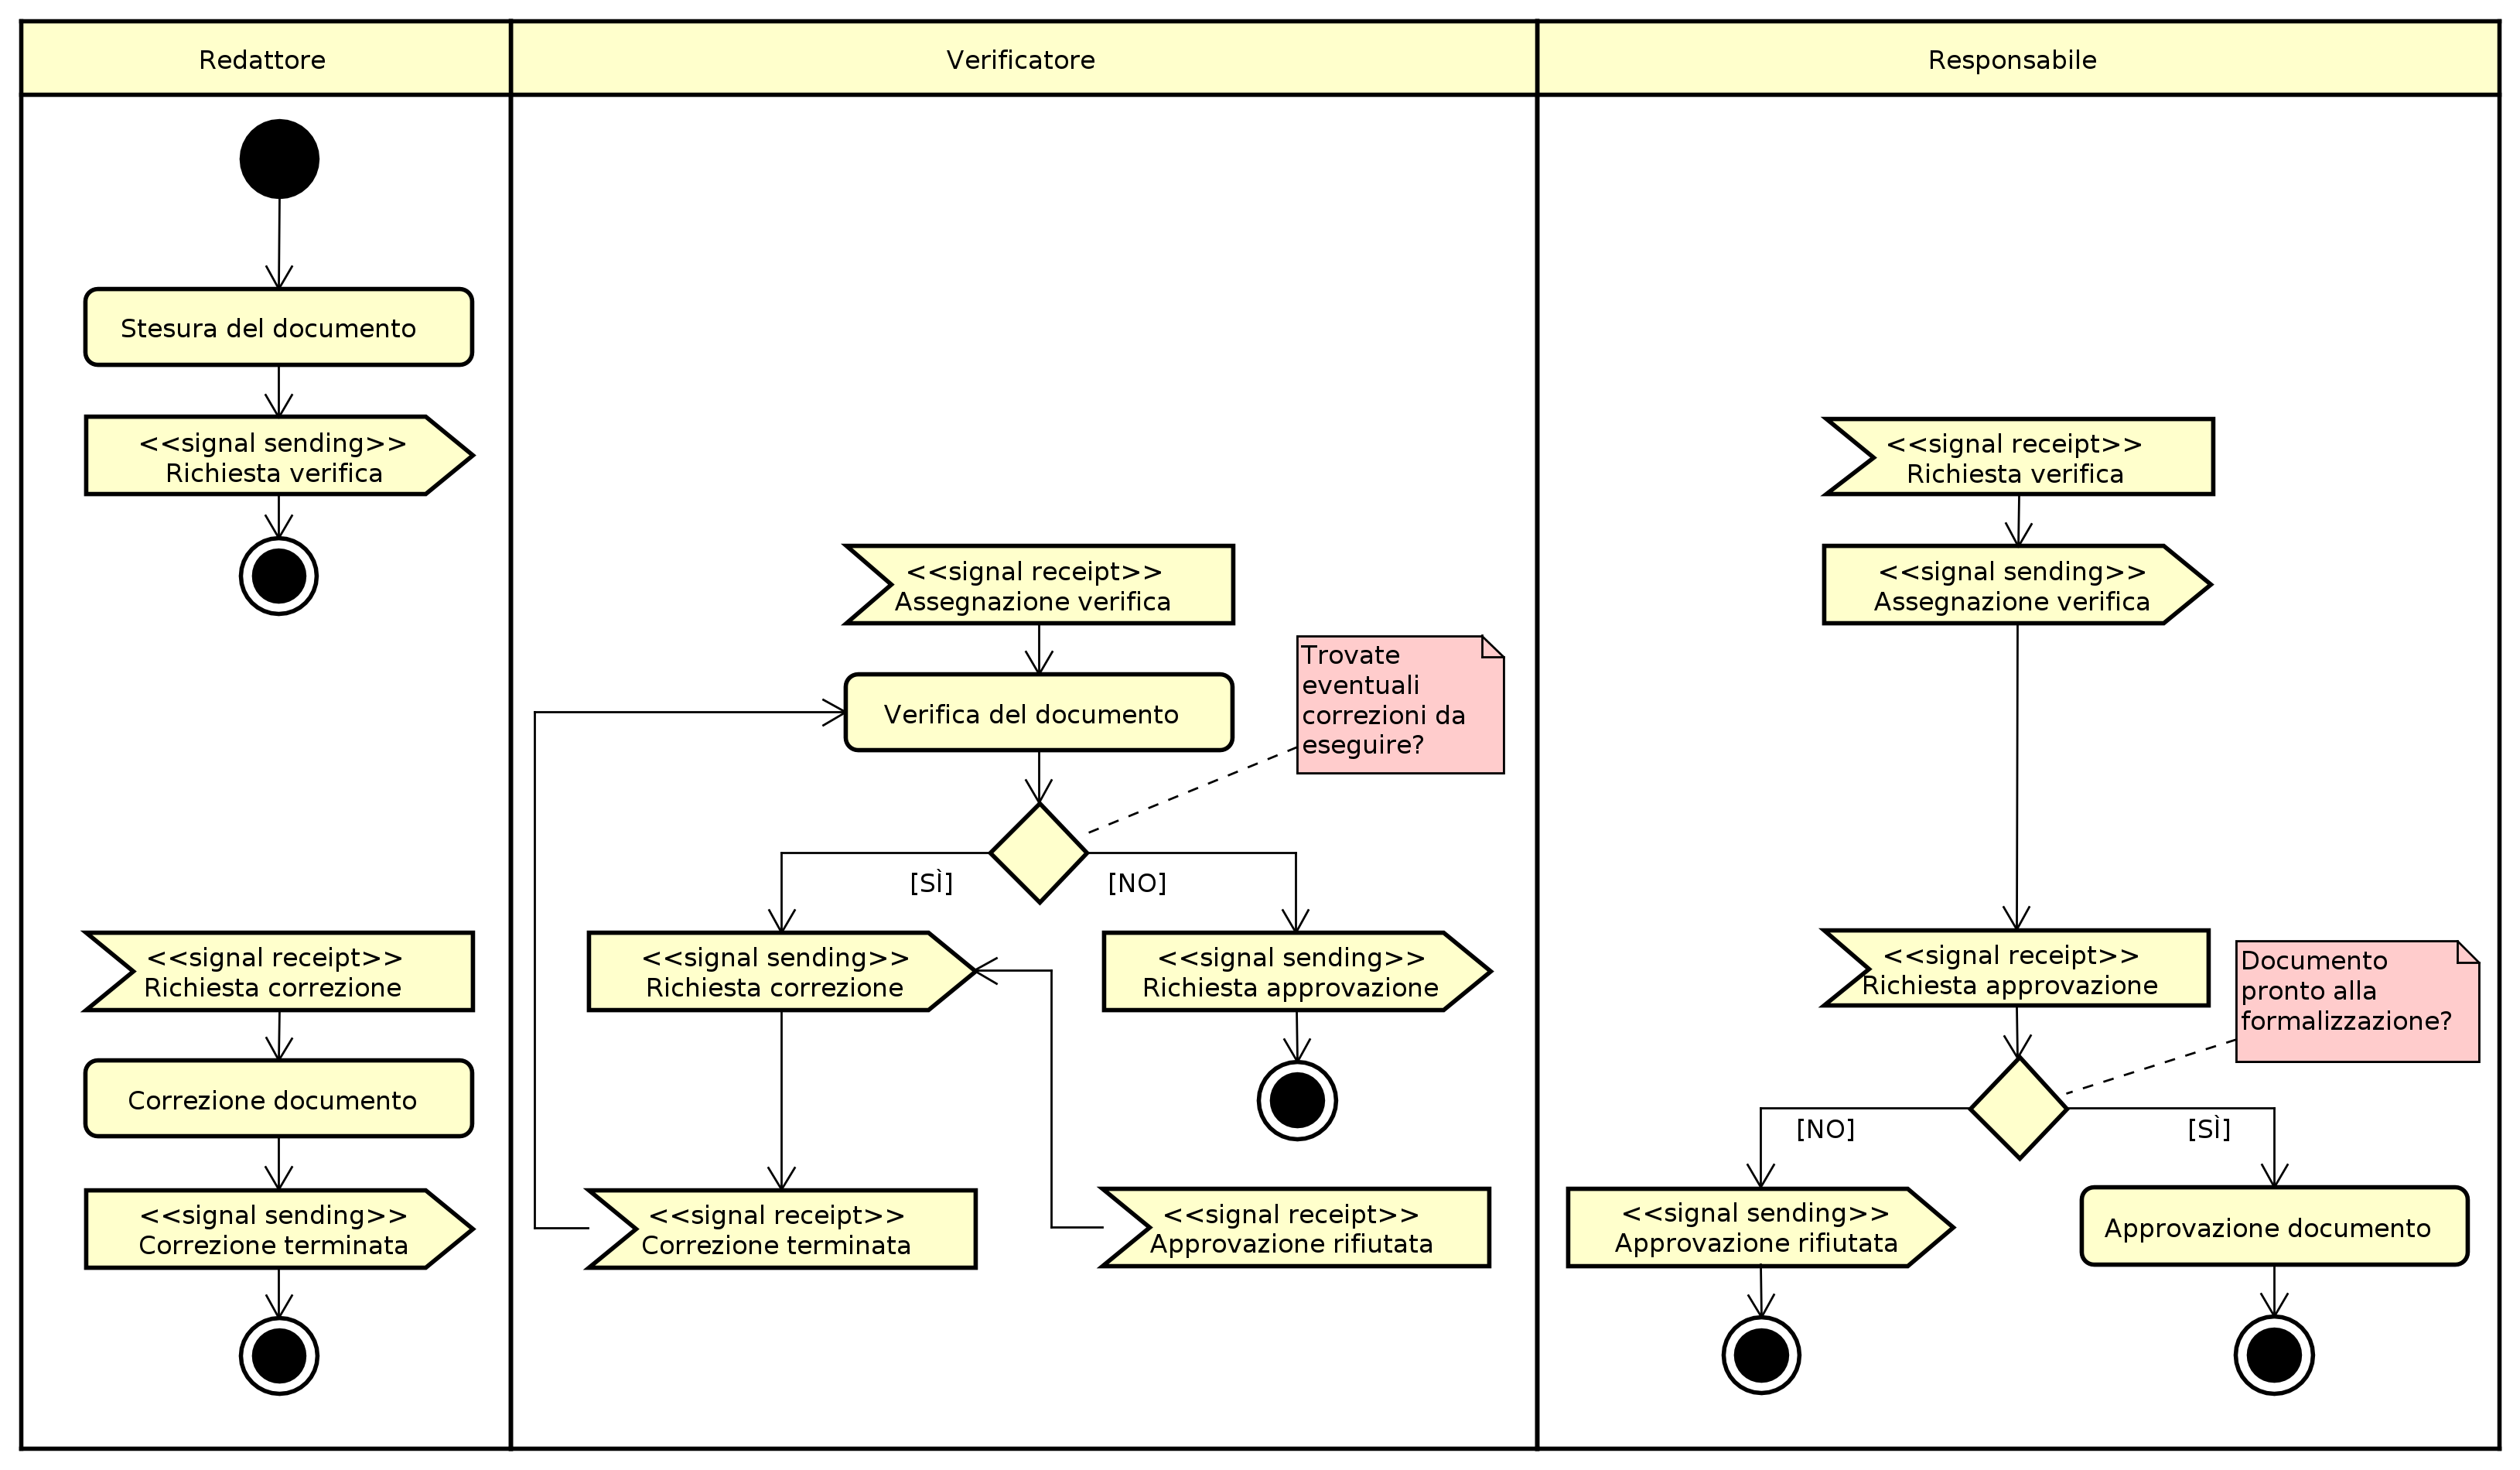
\includegraphics[width=\textwidth]{img/ciclo_di_vita_doc}
		        \caption{Ciclo di vita di un documento. Riferita nella sezione \ref{sec:ciclodivitadoc}}
                \label{fig:ciclovitadoc}
	        \end{figure}
	        
	        \paragraph{Aggiunta nuovi termini a glossario} \label{sec:insTermine}
	        Durante la stesura dei documenti, quando si ritiene che un termine debba essere inserito a glossario si deve seguire la seguente procedura:
	        \begin{enumerate}
	        	\item entrare nello spazio condiviso del gruppo su \glo{Google Drive}{Google Drive} (si veda sezione \ref{sec:GoogleDrive}) e aprire il foglio \texttt{Termini da inserire nel glossario};
	        	\item inserire il termine in fondo alla pagina.
	        \end{enumerate}
  
  \subsection{Gestione della configurazione}
  \subsubsection{Scopo}
        Lo scopo della gestione della configurazione è di individuare e gestire le parti che compongono i prodotti da realizzare (ovvero i Configuration Item, CI). La corretta implementazione del processo deve:
        \begin{itemize}
            \item individuare i CI;
            \item gestire la loro organizzazione all'interno del repository;
            \item gestire il versionamento.
        \end{itemize}

  \subsubsection{Repository}
  \paragraph{Struttura dei repository}
  Il gruppo ha scelto di utilizzare \glo{GitHub}{GitHub} per il versionamento e il salvataggio dei file inerenti le attività di progetto. L'\amministratore{} di progetto deve creare e organizzare i repository necessari e assicurarsi che tutti i membri del gruppo vi possano accedere. Ogni membro deve essere registrato su GitHub e aver attivato l'account studente.
  \newline \newline
  Il repository dedicato ai documenti si trova al seguente indirizzo:
  \begin{center}
  	\url{https://github.com/JordanGottardo/Documenti}
  \end{center}
  Il repository dedicato al codice si trova al seguente indirizzo:
  \begin{center}
  	\url{https://github.com/JordanGottardo/DeGeOp}
  \end{center}
  Le cartelle nel repository vengono organizzate nel seguente modo a partire dalla root:
  \begin{itemize}
  	\item \textbf{documenti:} sono presenti le cartelle per ogni revisione del progetto:
  	\begin{itemize}
  		\item \textbf{01-RR}: contenente i documenti e i file le necessari alla \revereq;
  		\item \textbf{02-RP}: contenente i documenti e i file le necessari alla \revprog;
  		\item \textbf{03-RQ}: contenente i documenti e i file le necessari alla \revaqual;
  		\item \textbf{04-RA}: contenente i documenti e i file le necessari alla \revacc;
  		\item \textbf{Script}: contenente script e altri strumenti utili per la stesura e la verifica dei documenti;
  		\item \textbf{Modello nuovo documento:} contenente i file con la struttura di base la creazione di un nuovo documento;
  		\item \textbf{Template}: contenente i file del template da usare per la creazione dei documenti \LaTeX.
  		\item \textbf{Consegne}: contenente i file delle consegne suddivise per revisione.
  	\end{itemize}
  	\item \textbf{codice}: la descrizione di questa cartella verrà fornita in un momento successivo.
  \end{itemize}
  
  \paragraph{Nomi dei file}
  I nomi dei documenti presenti nel repository devono rispettare la notazione \glo{Camel case}{camel case} con le seguenti caratteristiche:
  \begin{itemize}
  	\item la prima lettera di ogni file è maiuscola, le successive minuscole fino al presentarsi della parola successiva che inizia con la lettera maiuscola e cosi via;
  	\item è possibile utilizzare unicamente caratteri alfanumerici e il trattino basso;
  	\item i nomi non possono contenere spazi o elementi di punteggiatura.
  \end{itemize}

  \subsubsection{Versionamento}\label{sec:versionamento}
	  \paragraph{Controllo di versione}
	  Il controllo di versione del file sorgente, sia per il codice sia per i documenti, viene fatto utilizzando il software \glo{Git}{Git} e la piattaforma GitHub. 
	  \paragraph{Versionamento documenti}
		  Tutti i documenti devono essere identificati da una versione, ad ogni nuova versione deve corrispondere una riga nel registro delle modifiche.
		  La versione corrente di un documento deve sempre essere riportata all'interno dello stesso e va inoltre indicata in coda al nome del file con il seguente formato:\\\\
		  \centerline{\texttt{NomeDocumento\_vX.Y.Z.pdf}}
		  \begin{itemize}
		  	\item \textbf{X:}
		  	\begin{itemize}
		  		\item inizia da 0;
		  		\item viene incrementato solo dal \responsabilediprogetto, al momento della sua approvazione; 
		  		\item non può essere maggiore del numero di revisioni.
		  	\end{itemize}
		  	\item \textbf{Y:}
		  	\begin{itemize}
		  		\item inizia da 0;
		  		\item viene incrementato solo dai \verificatori{} ad ogni verifica eseguita;
		  		\item quando viene incrementato X, viene riportato a 0.
		  	\end{itemize}
		  	\item \textbf{Z:}
		  	\begin{itemize}
		  		\item inizia da 0;
		  		\item viene incrementato solo dai redattori al completamento di ogni task di modifica del documento;
		  		\item quando vengono incrementati X o Y, viene riportato a 0.
		  	\end{itemize}
		  \end{itemize}

		\paragraph{Versionamento applicazione}
		L'applicazione realizzata verrà versionata nel seguente modo:
		\begin{itemize}
			\item \textbf{X:}
			\begin{itemize}
				\item inizia da 0;
				\item viene incrementato solo dal \responsabilediprogetto, corrisponde all'ultima versione stabile del applicazione; 
				\item la versione 1 coinciderà con la revisione di accettazione.
			\end{itemize}
			\item \textbf{Y:}
			\begin{itemize}
				\item inizia da 0;
				\item viene incrementato solo dai \verificatori{} ad ogni incremento di funzionalità eseguito;
				\item quando viene incrementato X, viene riportato a 0.
			\end{itemize}
			\item \textbf{Z:}
			\begin{itemize}
				\item inizia da 0;
				\item viene incrementato solo dai \programmatori{} al completamento di ogni task di modifica;
				\item quando vengono incrementati X o Y, viene riportato a 0.
			\end{itemize}
		\end{itemize}
  
        \paragraph{Messaggi di commit}
        Ogni volta che si effettuano modifiche sui file del repository locale per poi esser caricate in quello remoto, bisogna specificarne le motivazioni. Per uniformare l'ambiente di lavoro è stato scelto un formato standard per la scrittura dei messaggi di \glo{Commit}{commit} che devono contenere:
        \begin{itemize}
            \item breve messaggio riassuntivo delle operazioni svolte;
            \item lista dei file modificati;
            \item lista delle modifiche per i singoli file.
        \end{itemize}
        Si veda la sezione \ref{sec:commit} per il dettaglio sulla procedura da seguire.
  
	  \subsubsection{Strumenti}
	  \paragraph{Git}
	  Git è un \glo{Sistema di controllo di versione}{sistema software di controllo di versione} distribuito e \glo{Open source}{open source}. La versione utilizzata al momento della stesura di questo documento è la 2.11.0 o superiore.
	  Le principali motivazioni che hanno portato il gruppo alla scelta di questo strumento sono:
	  \begin{itemize}
	  	\item ampio uso in ambito lavorativo;
	  	\item performance superiori rispetto ad altri sistemi di versionamento;
	  	\item sistema distribuito anziché centralizzato.
	  \end{itemize}
	  Indirizzo per il download e documentazione:
	  \begin{center}
	  	\url{https://git-scm.com}
	  \end{center}
	  L'utilizzo di Git verrà effettuato tramite riga di comando. Si lascia libertà ai membri del gruppo per l'installazione di eventuali interfacce grafiche personalizzate.
	  %
	  \paragraph{GitHub}
	  GitHub è un servizio web di hosting per lo sviluppo di progetti software. Tra le caratteristiche principali:
	  \begin{itemize}
	  	\item utilizzo del sistema di controllo di versione Git;
	  	\item possibilità di inserire documentazione e immagini, oltre al codice sorgente ;
	  	\item \glo{Issue}{issue} tracking;
	  	\item funzionalità simili ai social network come follower, commenti e notifiche;
	  	\item visione di grafici e statistiche su sviluppatori e repository.
	  \end{itemize}
	  Le principali motivazioni che hanno portato il gruppo alla scelta di questo strumento sono:
	  \begin{itemize}
	  	\item possibilità di creare repository private attivando il piano studente con l'email universitaria;
	  	\item sistema largamente diffuso e conosciuto da alcuni membri del gruppo;
	  	\item integrabile con altre applicazioni (es: \glo{Slack}{Slack}, \glo{IDE}{IDE}).
	  \end{itemize}
  
	  \subsubsection{Procedure}
	  \paragraph{Installazione e configurazione di Git}
	  L'installazione di Git varia a seconda del sistema operativo utilizzato. Di seguito verranno elencate le principali procedure d'installazione.
	  \newline \newline
	  Per i sistemi \glo{Linux}{Linux}:
	  \begin{itemize}
	  	\item aprire il terminale;
	  	\item eseguire il comando sudo \texttt{apt-get update};
	  	\item eseguire il comando \texttt{apt-get install git}.
	  \end{itemize}
	  Per i sistemi \glo{Windows}{Windows}:
	  \begin{itemize}
	  	\item accedere al sito ufficiale \url{https://git-scm.com/download/win};
	  	\item scaricare l'eseguibile;
	  	\item installare l'eseguibile seguendo la procedura guidata.
	  \end{itemize}
	  Per i sistemi \glo{MacOS}{MacOS}:
	  \begin{itemize}
	  	\item accedere al sito ufficiale \url{https://git-scm.com/download/mac};
	  	\item scaricare l'eseguibile;
	  	\item aprire il file appena scaricato e avviare l'installazione cliccando sul file \texttt{.pkg}.
	  \end{itemize}
	  La configurazione iniziale prevede l'inserimento del nome dell'utente e la connessione con l'account GitHub tramite la seguente procedura:
	  \begin{itemize}
	  	\item \texttt{{git} config --global user.name <Nome Cognome>}: imposta il nome dell'utente, che comparirà come autore delle commit effettuate;
	  	\item \texttt{{git} config --global user.email <email>}: imposta l'email dell'utente; deve essere impostata la stessa email utilizzata per la registrazione su GitHub.
	  \end{itemize}
	  Per la creazione di una cartella locale del repository si deve seguire la seguente procedura:
	  \begin{itemize}
	  	\item creare una nuova cartella;
	  	\item aprire il terminale;
	  	\item posizionarsi all'interno della cartella precedentemente creata;
	  	\item eseguire il comando: \texttt{git init};
	  	\item recuperare l'indirizzo URL del progetto su GitHub;
	  	\item eseguire il comando: \texttt{git clone <indirizzo appena recuperato>}.
	  \end{itemize}
	  \paragraph{Aggiornamento del repository} \label{sec:commit}
	  L'aggiornamento del repository deve essere svolto eseguendo i seguenti comandi:
	  \begin{enumerate}
	  	\item eseguire \texttt{git pull} per scaricare le modifiche da remoto;
	  	\item se sono presenti conflitti:
	  	\begin{enumerate}
	  		\item eseguire \texttt{git stash} per salvare momentaneamente le modifiche locali;
	  		\item eseguire \texttt{git pull};
	  		\item eseguire \texttt{git stash apply} per ripristinare le modifiche;
	  	\end{enumerate}
	  	\item eseguire \texttt{git add NomeFile} per ognuno dei file in cui sono state effettuate delle modifiche;
	  	\item eseguire \texttt{git commit -m "descrizione modifiche"};
	  	\item eseguire \texttt{git push} per inviare le modifiche al repository remoto.
	  \end{enumerate}
	  \begin{figure}[H]
	  	\centering
	  	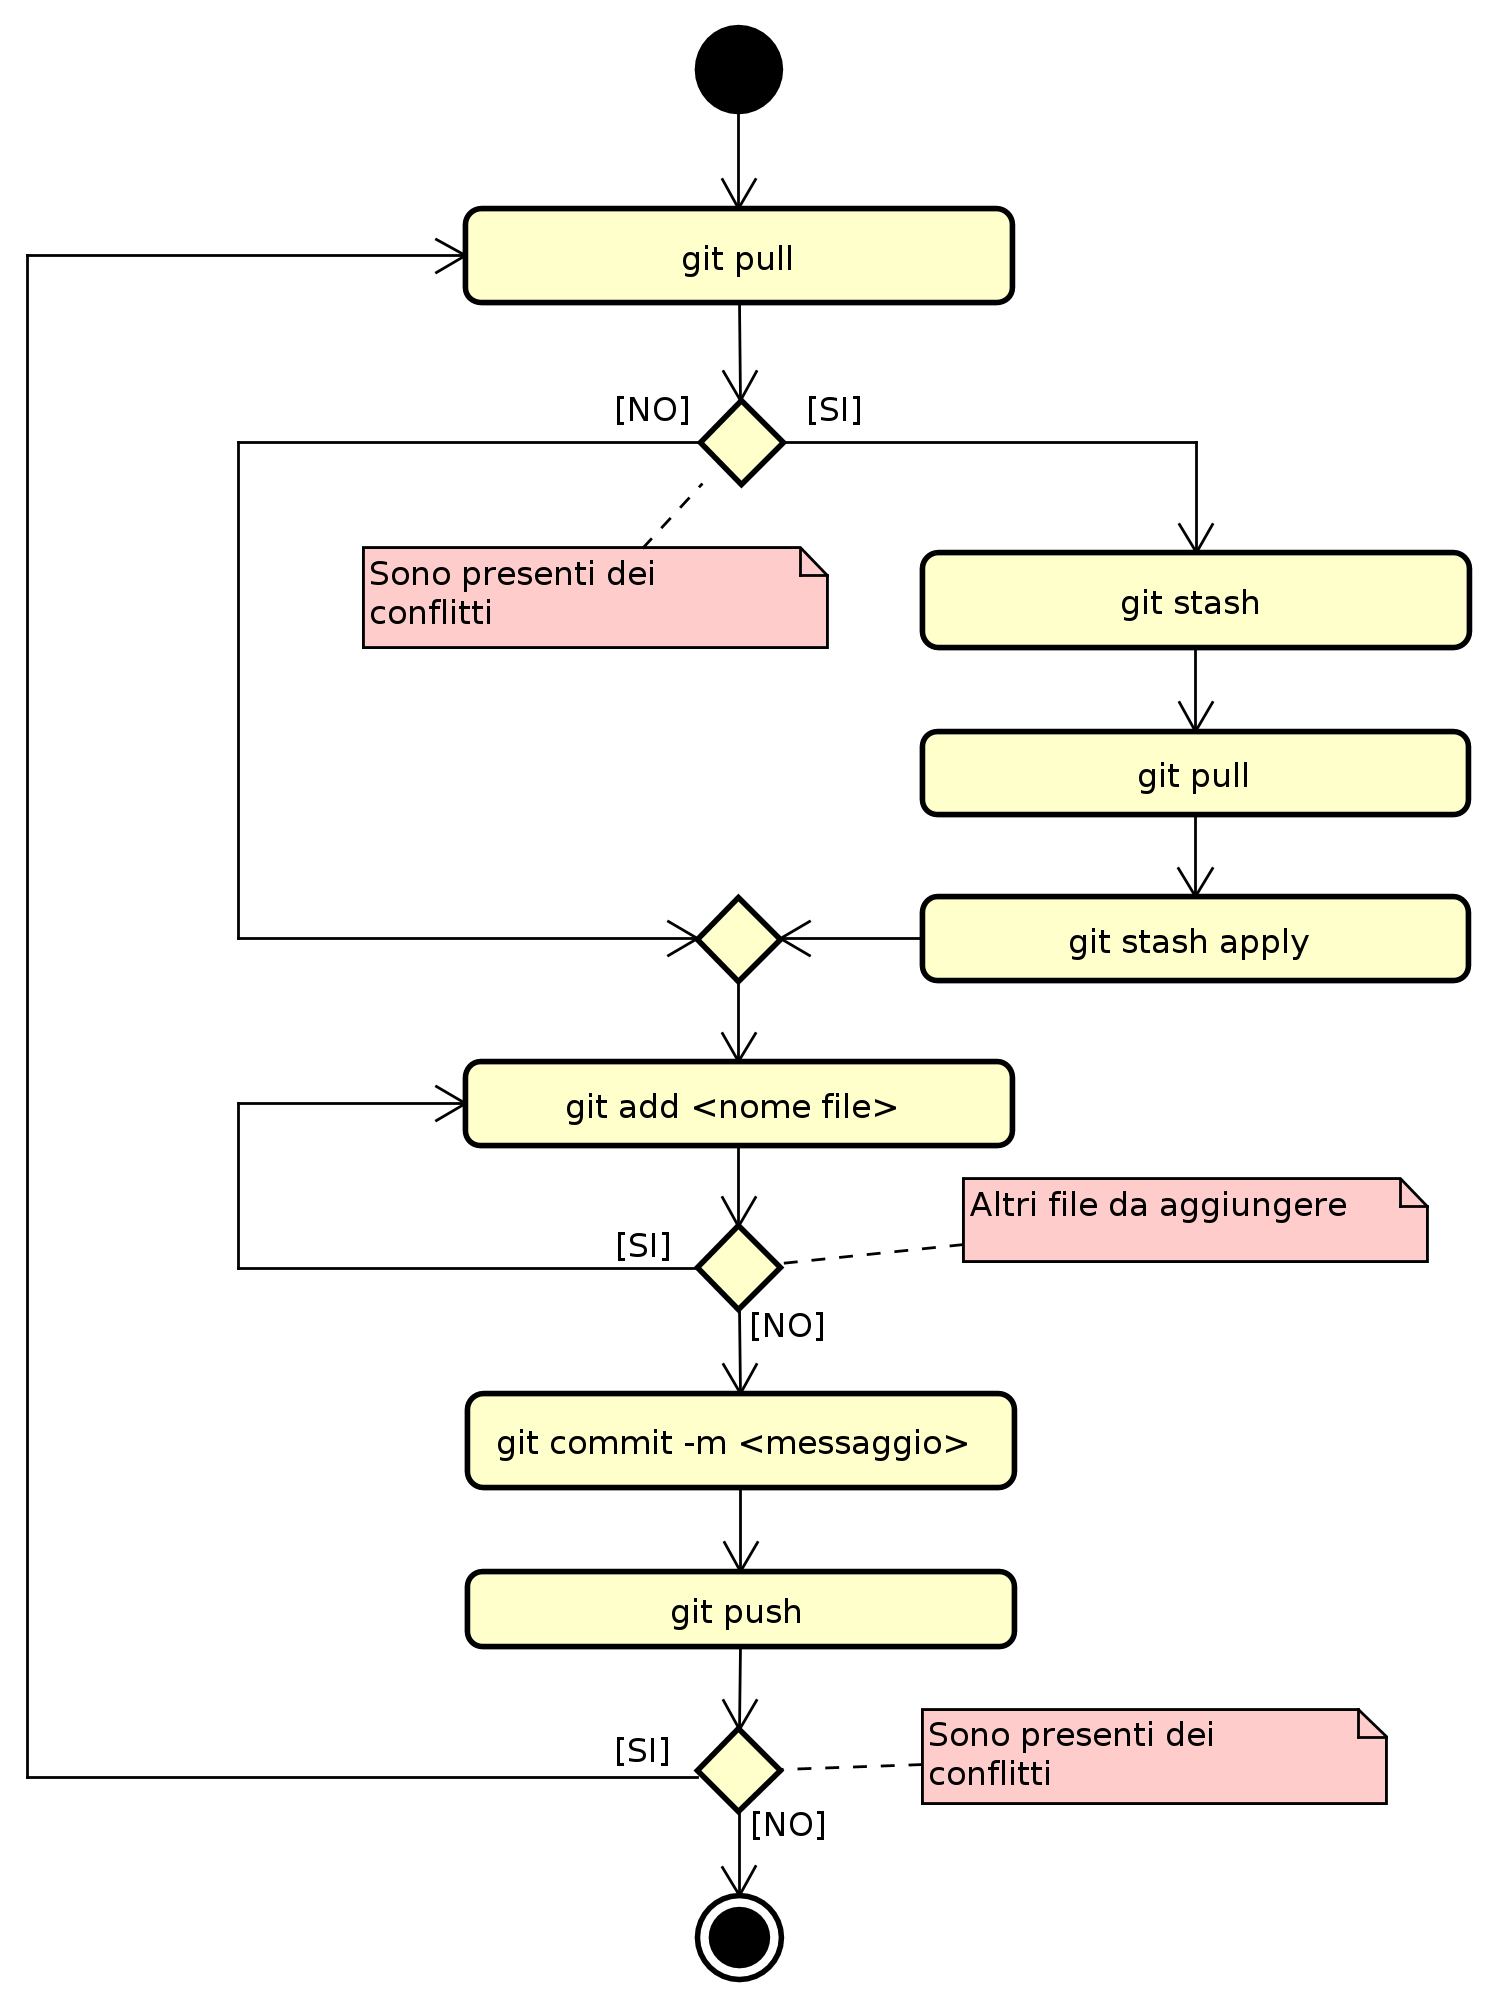
\includegraphics[width=0.7\textwidth]{img/AggiornamentoRepository}
	  	\caption{Procedura di aggiornamento del repository.}
	  \end{figure}
	  \paragraph{Comandi utili Git}
	  Per l'approfondimento dei principali comandi riguardanti l'utilizzo di Git è stata redatta una guida, consultabile al seguente indirizzo: \href{https://github.com/JordanGottardo/Documenti/blob/master/README.md}{Guida Git}.
	%
	
    \subsection{Verifica}\label{sec:verifica}
        \subsubsection{Scopo}
        Lo scopo del processo di verifica è di garantire che ogni attività dei processi svolti non introduca errori nel prodotto e che soddisfi i requisiti o le condizioni necessarie per essere considerata accettabile. La corretta implementazione del processo deve:
        \begin{itemize}
            \item fornire le procedure di verifica necessarie;
            \item individuare i criteri per la verifica;
            \item individuare eventuali difetti perchè possano essere corretti.
        \end{itemize}
		\subsubsection{Documenti} \label{sec:documenti}
		Il \responsabilediprogetto{} deve assegnare i compiti ai \verificatori, ognuno di essi deve effettuare un controllo accurato delle seguenti regole:
		\begin{itemize}
			\item devono essere rispettate le norme tipografiche (vedi sez. \ref{sec:normeTipografiche});
			\item devono essere rispettate le componenti grafiche (vedi sez. \ref{sec:normeGrafiche});
			\item devono essere rispettate le regole per i termini a glossario (vedi sez. \ref{sec:normeGlossario});
			\item devono essere utilizzati periodi brevi, corretti e il più possibile semplici;
			\item devono essere usati i comandi \LaTeX{} descritti nell'appendice \ref{ComandiLatex};
			\item deve essere rispettata la struttura del documento (vedi sez. \ref{sec:strutturaDoc}).
		\end{itemize}
	
		\subsubsection{Metriche}
			\paragraph{Processi}
				\subparagraph{Livello CMM ($LCMM$)} \label{LCMM}
				La metrica scelta è il Livello \glo{CMM}{CMM} (LCMM). La scala assume valori da 1 (peggiore) a 5 (migliore).
				%
				\subparagraph{Schedule Variance ($SV$)} \label{SV}
				La metrica utilizzata è la Schedule Variance (SV). È implementata come differenza tra la pianificazione dei costi del lavoro eseguito e del lavoro pianificato. Entrambi questi valori sono intesi nella loro accezione temporale (giorni) e non monetaria.
				$$SV = BCWP-BCWS$$
				dove $BCWP$=Budgeted Cost of Work Performed e $BCWS$=Budgeted Cost of Work Scheduled.
				%
				\subparagraph{Cost Variance ($CV$)} \label{CV}
				La metrica utilizzata è la Cost Variance (CV). È implementata come differenza tra costo pianificato e costo effettivo del lavoro eseguito.
				$$CV = BCWP-ACWP$$ dove $BCWP$=Budgeted Cost of Work Performed e $ACWP$=Actual Cost of Work Performed.
				%
				\subparagraph{Rischi Non Preventivati ($RNP$)} \label{RNP}
				È stato creato un contatore RNP (Rischi Non Preventivati) che aumenta di 1 ogni volta che si presenta un rischio non preventivato nel \pdpv. Il contatore rimane attivo durante tutto il ciclo di vita del progetto.
				%
				\subparagraph{Righe Documento Per Ora ($RDCO$)} \label{RDCO}
				È stato creato un contatore RDCO (Righe Documento Per Ora) che tiene conto delle righe di documento che vengono redatte da un membro del gruppo.
				$$RDCO=\frac{RP}{OI}$$ dove $RP$=Righe Prodotte e $OI$=Ore Impiegate nella scrittura del documento
				%
				\subparagraph{Numero Comandi Richiesti ($NCR$)} \label{NCR}
				È stato creato un contatore NCR (Numero Comandi Richiesti) che tiene conto dei comandi personalizzati per il template \LaTeX{} che vengono richiesti al \responsabilediprogetto.
				%
				\subparagraph{Risoluzione Verticale ($RV$)} \label{RV}
				Metrica che tiene conto dei pixel verticali di un'immagine.
				Come riferimento viene preso il valore di $RV$ minimo tra le immagini.
				%
				\subparagraph{Percentuale Tracciamento Modifiche ($PTM$)} \label{PTM}
				$$PTM=\frac{NTC}{NARM}$$
				dove $NTC$=Numero di Task Completati relativi ad un documento e $NARM$=Numero Aggiunte Registro Modifiche.
				%
				\subparagraph{Righe Codice Per Ora ($RCPO$)} \label{RCPO}
				$$RCPO=\frac{RC}{OI}$$
				dove $RC$=Righe di Codice scritte e $OI$=Ore Impiegate.
				%
				\subparagraph{Use Case senza Scenario Principale ($UCSP$)} \label{UCSP}
				Metrica che tiene conto del numero di use case senza scenario principale.
				%
				\subparagraph{Percentuale di Requisiti Obbligatori Coperti ($PROC$)} \label{PROC}
				$$PROC=\frac{ROC}{ROI}$$
				dove $ROC$=Requisiti Obbligatori Coperti, ovvero assegnati ad un \glo{Package}{package} e $ROI$=Requisiti Obbligatori Individuati.
				%
				\subparagraph{Grado di Accoppiamento ($GA$)} \label{GA}
				Metrica che indica le dipendenze uscenti delle componenti (package/classi) del sistema verso altre componenti. 
				Viene preso come riferimento il massimo $GA$ tra quelli presenti.
				%
				\subparagraph{Grado di Utilità ($GU$)} \label{GU}
				Metrica che indica le dipendenze entranti nelle componenti del sistema.
				Viene preso come riferimento il minimo $GU$ tra quelli presenti.
				%
			\paragraph{Documenti}
				\subparagraph{Indice Gulpease ($IG$)} \label{IG}
				La metrica utilizzata è l'\glo{Indice Gulpease}{Indice Gulpease} ($IG$), un indice di leggibilità di un testo tarato sulla lingua italiana. La scala va da 0 a 100, dove "0" indica un documento di bassa leggibilità e "100" uno di alta. Risulta che i testi con indice:
				\begin{itemize}
					\item inferiore a 80 sono difficili da leggere per chi ha la licenza elementare;
					\item inferiore a 60 sono difficili da leggere per chi ha la licenza media;
					\item inferiore a 40 sono difficili da leggere per chi ha un diploma superiore.
				\end{itemize}
				$$IG=89 + \frac{300\cdot{}NF-10\cdot{}NL}{NP}$$
				dove $NF$ è il Numero di Frasi, $NL$ è il Numero di Lettere e $NP$ è il Numero di Parole presenti nel testo.
				%
				\subparagraph{Errori riguardanti le Norme interne e Non Corretti ($ENNC$)} \label{ENNC}
				La metrica utilizzata è il numero di Errori riguardanti le Norme interne rinvenuti e Non Corretti ($ENNC$). È implementata con un contatore che aumenta di 1 ogni volta che un errore riguardante le norme interne rilevato da un \verificatore{} non viene corretto. Il contatore fa riferimento ad uno specifico \glo{Periodo}{periodo} e viene azzerato successivamente.
				%
				\subparagraph{Errori Ortografici Non Corretti ($EONC$)} \label{EONC}
				La metrica utilizzata è un contatore di Errori Ortografici Non Corretti ($EONC$), che aumenta di 1 ogni volta che un errore ortografico rilevato da un \verificatore{} non viene corretto. Il contatore fa riferimento ad uno specifico periodo e viene azzerato successivamente.
				%
				\subparagraph{Errori Concettuali Non Corretti ($ECNC$)} \label{ECNC}
				La metrica utilizzata è chiamata Errori Concettuali Non Corretti ($ECNC$). La formula è data dal complemento a 1 del rapporto tra errori concettuali corretti e rilevati. Tali errori possono essere rilevati dai Verificatori o dal committente.
				$$ECNC=\left(1-\frac{ECC}{ECR}\right)\cdot100$$
				dove $ECC$=Errori Concettuali Corretti e $ECR$=Errori Concettuali Rinvenuti.
				%
				\subparagraph{Livello Annidamento Indice ($LAI$)} \label{LAI}
				Metrica che conta il livello di annidamento dell’indice.
				Viene preso come riferimento il massimo $LAI$ tra quelli presenti.
				
			\paragraph{Codice}
				\subparagraph{Implementazione delle Funzionalità Obbligatorie ($IFO$)} \label{IFO}
				La metrica utilizzata è chiamata Implementazione delle Funzionalità Obbligatorie ($IFO$). Essa consiste in un rapporto tra il numero di requisiti obbligatori soddisfatti e identificati
				$$IFO= \frac{ROS}{ROI}\cdot 100$$
				dove $ROS$=numero di Requisiti Obbligatori Soddisfatti e $ROI$=numero di Requisiti Obbligatori Identificati.
				%
				\subparagraph{Implementazione delle Funzionalità Desiderabili ($IFD$)} \label{IFD}
				La metrica utilizzata è chiamata Implementazione delle Funzionalità Desiderabili ($IFD$). Essa consiste in un rapporto tra il numero di requisiti desiderabili soddisfatti e identificati
				$$IFD= \frac{RDS}{RDI}\cdot 100$$
				dove $RDS$=numero di Requisiti Desiderabili Soddisfatti e $RDI$=numero di Requisiti Desiderabili Identificati.
				%
				\subparagraph{Numero di Statement per Metodo ($NSM$)} \label{NSM}
				Metrica che conta il Numero di \glo{Statement}{Statement} per Metodo.
				Viene preso come riferimento il massimo $NSM$ tra quelli presenti.
				%
				\subparagraph{Numero di Parametri per Metodo ($NPM$)} \label{NPM}
				Metrica che conta il Numero di Parametri per Metodo.
				Viene preso come riferimento il massimo $NPM$ tra quelli presenti.
				%
				\subparagraph{Numero Campi Dati Per Classe ($NCDPC$)} \label{NCDPC}
				Metrica che conta il Numero di Campi Dati per Classe.
				Viene preso come riferimento il massimo $NCDPC$ tra quelli presenti.
				%
				\subparagraph{Numero Ciclomatico ($NC$)} \label{NC}
				La metrica è basata sul Numero Ciclomatico ($NC$). Il conteggio viene fatto a livello di metodo.
				$$NC=e-n+2p$$
				dove $e$=numero di archi, $n$=numero di nodi, $p$=numero di componenti connesse.\\
				Viene preso come riferimento il massimo $NC$ tra quelli presenti.
				%
				\subparagraph{Numero di Variabili dichiarate e Non Utilizzate ($NVNU$)} \label{NVNU}
				Metrica che conta il numero di variabili dichiarate e non utilizzate.
				%
				\subparagraph{Rapporto tra le linee di Commento e le linee di Codice ($RCC$)} \label{RCC}
				La metrica è implementata come Rapporto tra le linee di Commento e le linee di Codice ($RCC$).
				$$RCC=\left(\frac{LDCM}{LDCC}\right)\cdot 100$$
				dove $LDCC$=Linee Di Codice e $LDCM$=Linee Di Commento.
				%
				\subparagraph{Superamento dei Test Pianificati ($STP$)} \label{STP}
				La metrica utilizzata è il Superamento dei Test Pianificati ($STP$). I test presi in considerazione sono quelli necessari a verificare l'implementazione delle funzionalità previste dai requisiti.
				$$STP=\frac{TS}{TP}\cdot100$$
				dove $TS$=numero di Test Superati e $TP$=numero di Test Pianificati.
				%
				\subparagraph{Breakdown Avoidance ($BA$)} \label{BA}
				La metrica utilizzata è la Breakdown Avoidance ($BA$).
				$$BA=\left( 1-\frac{NI}{NSA} \right)\cdot 100$$
				dove $NI$=Numero di Interruzioni e $NSA$=Numero di Situazioni Anomale.
				%
				\subparagraph{Failure Avoidance ($FA$)} \label{FA}
				La metrica utilizzata è la Failure Avoidance ($FA$).
				$$FA=\left(\frac{SAE}{SAT}\right) \cdot 100$$
				dove $SAE$=Situazioni Anomale Evitate e $SAT$=Situazioni Anomale Testate.
				%
				\subparagraph{Statement Coverage ($SC$)} \label{SC}
				Metrica utilizzata per calcolare la copertura degli statement.
				$$SC=\frac{NSE}{NSM}$$
				dove $NSM$=Numero Statement del Metodo e $NSE$=Numero Statement Eseguiti dal test.
				Viene preso come riferimento il minimo $SC$ tra quelli presenti.
				%
				\subparagraph{Branch Coverage ($BC$)} \label{BC}
				Metrica utilizzata per calcolare la copertura dei flussi logici.
				$$BC=\frac{NFLT}{NFLM}$$
				dove $NFLT$=Numero di Flussi Logici del Metodo Testati e $NFLM$=Numero di Flussi Logici del Metodo.
				Viene preso come riferimento il minimo $BC$ tra quelli presenti.
		
		%\subsubsection{Test}
		
		\subsubsection{Strumenti}
		\paragraph{Tabella metriche processo-strumenti}
		\begin{table}[H]
			\centering
			\label{tab:metriceProcStrumenti}
			\begin{tabular}{cl}
				\toprule
				Metrica & Strumento \\
				\hline
				\hyperref[LCMM]{LCMM}    &  Procedura interna \ref{sec:lcmm} \\
				\hyperref[SV]{SV}      & \glo{Teamwork}{Teamwork}, vedi la sezione \ref{sec:procTicket}  \\
				\hyperref[CV]{CV}      & Teamwork, vedi sezione \ref{sec:procTicket}\\
				\hyperref[RNP]{RNP}     & Procedura interna \ref{sec:rnp} \\
				\hyperref[RDCO]{RDCO}    & Script interno, vedi procedura \ref{sec:loc} \\
				\hyperref[NCR]{NCR}     & Procedura interna \ref{sec:procRichieste} \\ 
				\hyperref[RV]{RV}      & Script interno, vedi procedura \ref{sec:imageRes} \\
				\hyperref[PTM]{PTM}     & Procedura interna \ref{sec:chiusuraticket}          \\
				\hyperref[RCPO]{RCPO}    & Script interno, vedi procedura \ref{sec:loc} \\ 
				\hyperref[UCSP]{UCSP}    & Statistiche \hyperref[sec:trender]{Trender} \\
				\hyperref[PROC]{PROC}    & Statistiche Trender \\
				\hyperref[GA]{GA} 		& Statistiche Trender \\
				\hyperref[GU]{GU}      & Statistiche Trender \\
				\bottomrule    
			\end{tabular}
			\caption{Tabella metriche processo-strumenti}
		\end{table}
		%
		\paragraph{Tabella metriche documenti-strumenti}
		\begin{table}[H]
			\centering
			\label{tab:metriceDocStrumenti}
			\begin{tabular}{cl}
				\toprule
				Metrica & Strumento \\
				\hline
				\hyperref[IG]{IG}    &  Script interno, vedi procedura \ref{sec:calcoloGulpease} \\
				\hyperref[ENNC]{ENCC} & Procedura interna \ref{sec:gestioneanomalie} \\
				\hyperref[EONC]{EONC} & Procedura interna \ref{sec:gestioneanomalie} \\
				\hyperref[ECNC]{ECNC} & Procedura interna \ref{sec:gestioneanomalie} \\
				\hyperref[LAI]{LAI} & Script interno, vedi procedura \ref{sec:ssPar} \\
				\bottomrule    
			\end{tabular}
			\caption{Tabella metriche documenti-strumenti}
		\end{table}
		%
		\paragraph{Tabella metriche codice-strumenti}
		\begin{table}[H]
			\centering
			\label{tab:metriceCodiceStrumenti}
			\begin{tabular}{cl}
				\toprule
				Metrica & Strumento \\
				\hline
				\hyperref[IFO]{IFO}		& Statistiche \hyperref[sec:trender]{Trender} \\
				\hyperref[IFD]{IFD}		& Statistiche Trender \\
				\hyperref[NSM]{NSM}		& \hyperref[sec:JSMeter]{JSMeter} \\
				\hyperref[NPM]{NPM}		& \hyperref[sec:ESLint]{ESLint} \\
				\hyperref[NCDPC]{NCDPC}	& Statistiche Trender \\
				\hyperref[NC]{NC}		& JSMeter \\
				\hyperref[NVNU]{NVNU} 	& ESLint \\
				\hyperref[RCC]{RCC}		& \hyperref[JSMeter]{JSMeter} \\
				\hyperref[STP]{STP}		& Statistiche \hyperref[par:trender]{Trender} \\
				\hyperref[BA]{BA}		& \hyperref[sec:Jasmine]{Jasmine} \\
				\hyperref[FA]{FA}		& Jasmine \\
				\hyperref[SC]{SC}		& \hyperref[sec:WebStorm]{WebStorm} tramite \hyperref[sec:Karma]{Karma} e \hyperref[sec:Istanbul]{Istanbul} \\
				\hyperref[BC]{BC}		& WebStorm tramite Karma e Istanbul \\
				\bottomrule    
			\end{tabular}
			\caption{Tabella metriche codice-strumenti}
		\end{table}
		\paragraph{Verifica ortografica}
		Viene utilizzato il correttore in tempo reale integrato nell'applicazione \glo{TeXstudio}{TeXstudio} descritta nella sezione \ref{sec:texstudio}. Il correttore identifica e sottolinea eventuali refusi ortografici; un'analisi più approfondita del testo è compito dei \verificatori.
		%
		\paragraph{Indice leggibilità} \label{sec:gulpease}
		La valutazione dell'indice di leggibilità è fatta secondo l'\glo{Indice Gulpease}{indice Gulpease} utilizzando uno script creato appositamente e fornito assieme al template. Lo script può analizzare sia il file sorgente scritto in \TeX{} che il file pdf risultante.
		%
		\paragraph{Analisi statica}
		\subparagraph{ESLint} \label{sec:ESLint}
		ESLint è un tool che permette di effettuare analisi statica su file \glo{JavaScript}{JavaScript} con lo scopo di ottenere codice più uniforme e privo di errori. I controlli che effettua sul codice vengono realizzati nei confronti di un insieme di regole personalizzabili, regole che gli sviluppatori possono attivare o disattivare in base alle loro guide di stile di codifica interna (vedi sezione: \ref{sec:stileCodifica}). \\
		La documentazione e l'installazione di ESLint sono disponibili al seguente indirizzo:
		\begin{center}
			\url{https://github.com/eslint/eslint}
		\end{center}
		%
		\subparagraph{JSMeter} \label{sec:JSMeter}
		JSMeter è uno strumento che permette di calcolare diversi indici di misurazione della complessità del codice JavaScript descritti nel \pdqv.
		La documentazione e l'installazione di JSMeter sono disponibili al seguente indirizzo:
		\begin{center}
			\url{http://jsmeter.info}
		\end{center}
		%
		\paragraph{Analisi dinamica}
		\subparagraph{Karma}\label{sec:Karma}
		Karma è un ambiente di testing, utile ad effettuare test su browser e dispositivi. Per descrivere i test vengono utilizzati dei framework esterni, come per esempio Mocha o Jasmine. Karma viene utilizzato assieme ad un framework per l'esecuzione dei test di unità. \\
		La documentazione e l'installazione di Karma sono disponibili al seguente indirizzo:
		\begin{center}
			\url{https://github.com/karma-runner/karma}
		\end{center}
		%
		\subparagraph{Jasmine}\label{sec:Jasmine}
		\glo{Jasmine}{Jasmine} è un framework per implementare test di codice \js, non dipendendo da browser o altri framework è adatto ad eseguire test di siti web ed è facilmente estendibile. Oltre a mettere a disposizione un set di operazioni di confronto permette anche di utilizzare driver e stub. I test implementati possono essere eseguiti tramite l'inserimento del codice in uno specifico file html o utilizzando un test runner esterno come Karma.
		La documentazione e l'installazione di Jasmine sono disponibili al seguente indirizzo:
		\begin{center}
			\url{https://jasmine.github.io/index.html}
		\end{center}
		%
		\subparagraph{Istanbul}\label{sec:Istanbul}
		Instanbul è uno strumento che permette di calcolare alcune metriche di complessità del codice JavaScript descritte nel \pdqv{} e verrà installato come modulo per \glo{Node.js}{Node.js}.
		La documentazione e l'installazione di Istanbul sono disponibili al seguente indirizzo:
		\begin{center}
			\url{https://github.com/gotwarlost/istanbul}
		\end{center}
		%
		%		        \subparagraph{Mocha}
		%		        Mocha è un framework per l’esecuzione di test JavaScript; permette l'esecuzione di test asincroni ed in serie, consentendo segnalazioni flessibili ed accurate.\\
		%		        La documentazione e l'installazione di Mocha è raggiungibile al seguente indirizzo:
		%		        \begin{center}
		%		        	\url{https://github.com/mochajs/mocha}
		%		        \end{center}
		%		        %
		%		        \subparagraph{Enzyme}
		%		        Enzyme è un tool di testing JavaScript per React che permette di testare facilmente il DOM; va abbinato alla libreria Chai.\\
		%		        La documentazione e l'installazione di Enzyme è raggiungibile al seguente indirizzo:
		%		        \begin{center}
		%		        	\url{https://github.com/airbnb/enzyme/}
		%		        \end{center}
		%		        %
		%		        \subparagraph{Chai}
		%		        Chai è una libreria per gestire le asserzioni. Viene utilizzata assieme a molti framework di test per JavaScript.\\
		%		        La documentazione e l'installazione di Chai sono disponibili al seguente indirizzo:
		%		        \begin{center}
		%		        	\url{https://github.com/chaijs/chai}
		%		        \end{center}
		%		        %
		%		        \subparagraph{Sinon}
		%		        Sinon è un framework che fornisce spie, stub e mock per creare e svolgere i test di unità.
		%		        La documentazione e l'installazione di Sinon sono disponibili al seguente indirizzo:
		%		        \begin{center}
		%		        	\url{https://github.com/sinonjs/sinon}
		%		        \end{center}
		
        \subsubsection{Procedure}
	        \paragraph{Attività manuale di verifica}
	        Ogni attività manuale di verifica deve essere accompagnata da un resoconto (si veda la sez. \ref{sec:gestioneanomalie} per i dettagli). Per svolgere l'attività di verifica, il \verificatore{} deve rispettare le seguenti indicazioni:
	        \begin{enumerate}
	        	\item aprire il file sorgente da verificare (se è un documento, anche il file pdf);
	        	\item annotare gli errori rilevati da correggere;
	        	\item inserire nel codice sorgente uno dei seguenti commenti:
		        	\begin{itemize}
		        		\item TODO per segnalare un'aggiunta da eseguire al codice;
		        		\item FIXME per segnalare un errore rilevato per cui è stata proposta una soluzione;
		        		\item BUG per segnalare un'anomalia da rivedere e correggere;
		        	\end{itemize} 
	        	\item se è un documento, calcolare indice gulpease (vedi sez. \ref{sec:gulpease}) e riportare l'esito nel resoconto;
	        	\item aprire un subticket come riportato nella sez. \ref{sec:gestioneanomalie} riportando gli errori.
	        \end{enumerate}
    
            \paragraph{Analisi}
                \subparagraph{Analisi statica}
                Tecnica utilizzata per l'analisi e la verifica del codice sorgente e della documentazione associata. Può essere applicata secondo due strategie:
                \begin{itemize}
                    \item \textbf{\glo{Walkthrough}{walkthrough}:} lettura completa del codice sorgente da analizzare. Va utilizzata unicamente durante il primo periodo del progetto in quanto risulta onerosa e non efficiente. Gli \analisti{} che la utilizzano devono stilare una lista di controllo con gli errori rilevati più frequentemente;
                    \item \textbf{\glo{Inspection}{inspection}:} lettura mirata del codice sorgente da analizzare. È necessario avere una lista di controllo per poter localizzare eventuali punti critici in cui cercare errori. Dopo ogni analisi la lista di controllo deve essere incrementata con eventuali nuovi errori rilevati.
                \end{itemize}
                \subparagraph{Analisi dinamica}
                Tecnica per l'analisi del prodotto software, richiede l'esecuzione del programma e viene eseguita tramite dei test che verificano il funzionamento del prodotto. I test devono essere ripetibili e a parità di condizioni iniziale e ambiente devono fornire lo stesso output. Per ogni test deve quindi essere definito:
                \begin{itemize}
                    \item \textbf{ambiente:} sistema hardware e software in cui viene eseguito il test;
                    \item \textbf{stato iniziale:} stato iniziale da cui si parte ad eseguire il test;
                    \item \textbf{input:} input inserito;
                    \item \textbf{output:} output atteso.
                \end{itemize}
            
            \paragraph{Task di verifica}\label{sec:taskverifica}
            La gestione dei task di verifica avviene tramite la creazione di ticket nell'applicazione \glo{Teamwork}{Teamwork} che viene descritta nella sezione \ref{sec:teamwork}. \\
	        Al termine di ogni ticket il \responsabilediprogetto{} dovrà seguire la seguente procedura:
            \begin{enumerate}
                \item creare un ticket di verifica con i riferimenti al task da verificare e contrassegnarlo con la dicitura \cit{[VERIFICA]};
                \item assegnare il ticket creato ad un \verificatore;
                \item al completamento del ticket di verifica contrassegnare il ticket originale con la dicitura \cit{[VERIFICATO]}.
            \end{enumerate}
            Vedi anche figura \ref{fig:verificagestione}. \\

            \paragraph{Gestione delle anomalie}\label{sec:gestioneanomalie}
            La gestione delle anomalie durante il processo di verifica avviene tramite la creazione di ticket nell'applicazione Teamwork che viene descritta nella sezione \ref{sec:teamwork}. Nel caso in cui un \verificatore{} dovesse trovare delle anomalie durante un task di verifica queste dovranno essere gestite nel seguente modo:
            \begin{enumerate}
                \item deve essere creato un subticket contrassegnato da uno dei seguenti tag, questi saranno utilizzati in un secondo momento per il calcolo delle relative metriche:
                \begin{itemize}
                	\item \cit{[EN]} se l'anomalia riguarda il rispetto delle norme (vedi metrica \ref{ENNC});
                	\item \cit{[EO]} se l'anomalia riguarda un errore ortografico (vedi metrica \ref{EONC});
                	\item \cit{[EC]} se l'anomalia riguarda un errore concettuale (vedi metrica \ref{ECNC});
                	\item \cit{[ERR]} se l'anomalia non riguarda nessuno dei campi precedenti.
                \end{itemize}
                \item assegnare i subticket creati agli assegnatari del task di cui si sta eseguendo la verifica;
                \item al completamento di tutti i subticket chiudere il ticket di verifica.
            \end{enumerate}
            Vedi anche figura \ref{fig:verificagestione}.

            \begin{figure}[H]
		        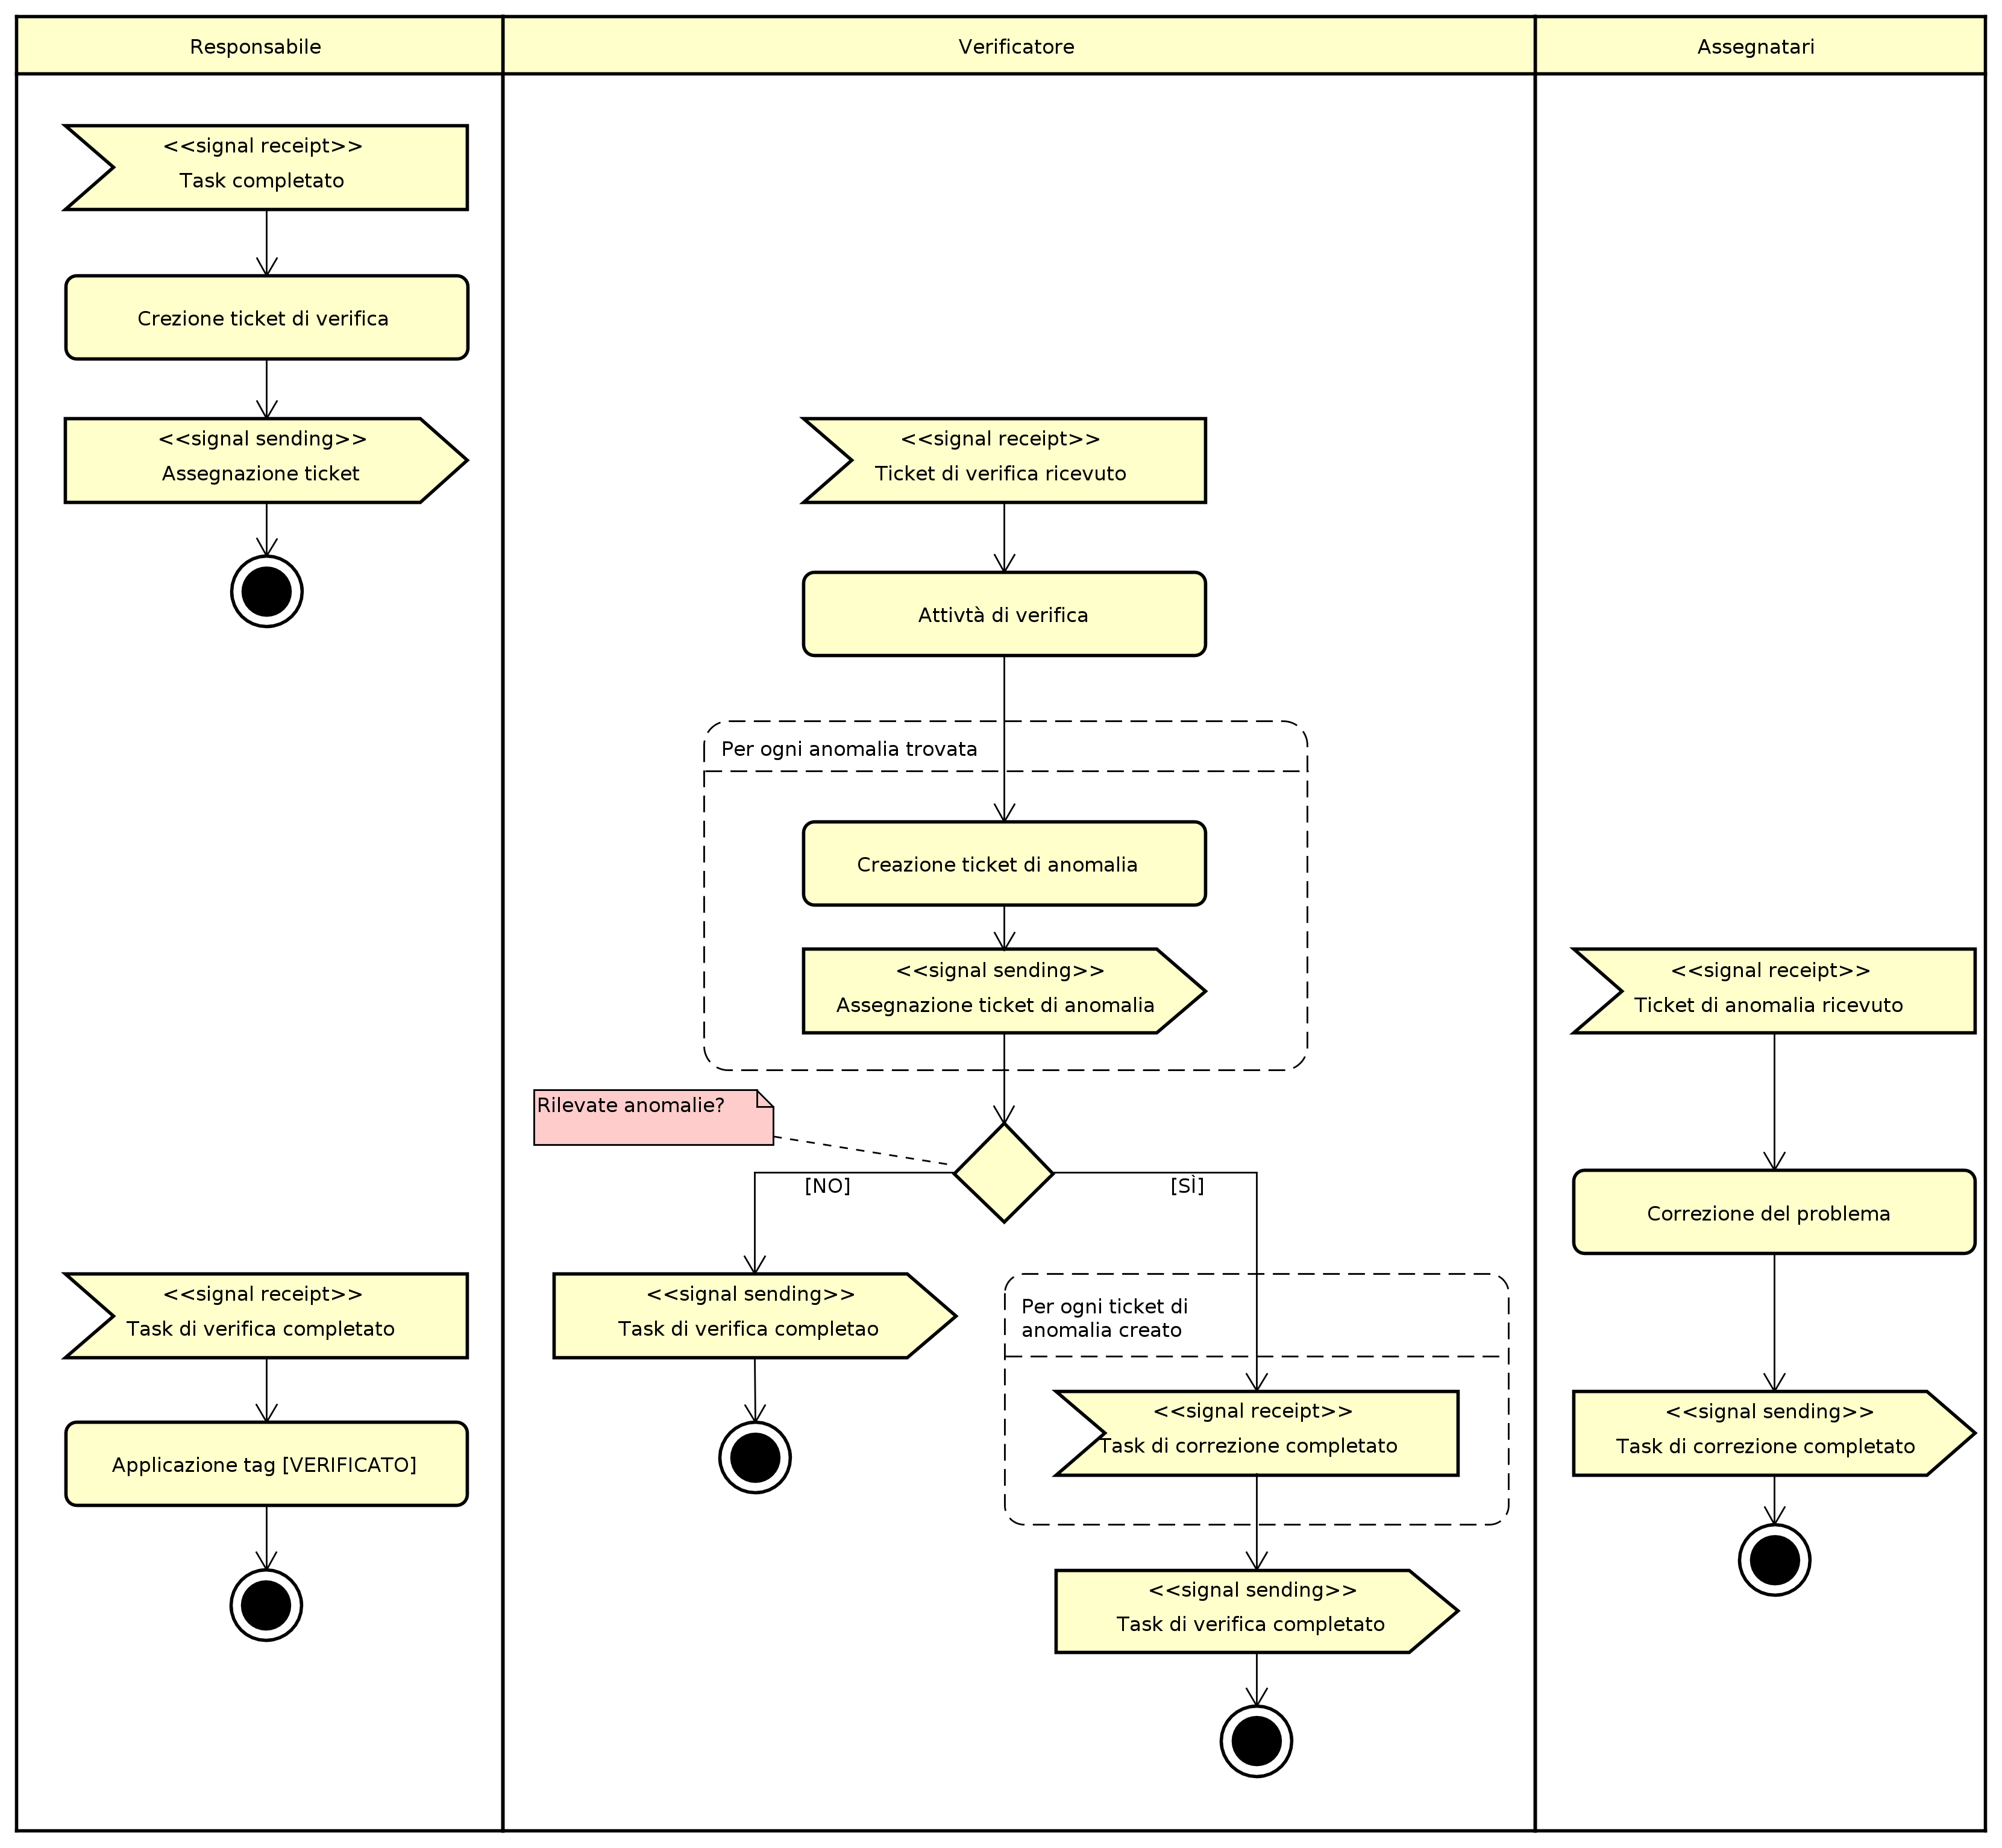
\includegraphics[width=\textwidth]{img/verifica_gestione_task}
		        \caption{Procedura di verifica dei task e gestione delle anomalie. Riferita nelle sezioni \ref{sec:taskverifica} e \ref{sec:gestioneanomalie}}
                \label{fig:verificagestione}
	        \end{figure}
	        %
	        \paragraph{Calcolo CMM}\label{sec:lcmm}
	        Al termine di ogni periodo il \responsabilediprogetto{} ha il compito di individuare il livello CMM che si è raggiunto. La decisione deve essere presa tenendo in considerazione:
	        \begin{itemize}
	        	\item le norme prodotte fino a quel momento ed il loro rispetto;
	        	\item i processi svolti, i loro risultati e la loro riproducibilità;
	        	\item le metriche individuate ed i loro valori.
	        \end{itemize} 
	        %
	        \paragraph{Calcolo rischi non preventivati}\label{sec:rnp}
	        Al momento di attualizzare un rischio il \responsabilediprogetto{} deve verificare che tale rischio sia presente nel \pdp{}. Se così non fosse dovrà procedere nel seguente modo:
	        \begin{itemize}
	        	\item creare un task ed inserire nel titolo il tag \cit{[RISK]};
	        	\item scrivere nella descrizione del task il rischio riscontrato;
	        	\item assegnare il task ad un analista responsabile del \pdp{} in modo che sia inserito nel documento.
	        \end{itemize}
	        Il \responsabilediprogetto{} dovrà tenere traccia dei ticket creati con il tag \cit{[RISK]} per calcolare il valore della metrica.
	        %
	        \paragraph{Calcolo dell'indice Gulpease} \label{sec:calcoloGulpease}
	        Per l'esecuzione dello script per il calcolo dell'indice Gulpease (descritto nella sezione \ref{sec:gulpease}) si dovranno seguire i seguenti passi:
	        \begin{enumerate}
	        	\item aprire una riga di comando o terminale;
	        	\item posizionarsi nella cartella \texttt{/script} all'interno dello spazio di lavoro condiviso \glo{Dropbox}{Dropbox};
	        	\item eseguire il comando: \texttt{gulpeasepdf.pl NomeDocumento.pdf};
	        	\item copiare l'esito prodotto dall'output del terminale.
	        \end{enumerate}
	        %
	        \paragraph{Calcolo linee modificate} \label{sec:loc}
	        \begin{enumerate}
	        	\item aprire una riga di comando o terminale;
	        	\item posizionarsi nella cartella \texttt{/script} all'interno del repository desiderato (Documenti o DeGeOp);
	        	\item eseguire il comando \texttt{git pull} per assicurarsi che il repository sia aggiornato;
	        	\item eseguire il comando: \texttt{./checkLOCgit.sh [-d numero\_giorni]};
	        	\item le immagini segnalate dal comando non rispettano la metrica.
	        \end{enumerate}
	        %
	        \paragraph{Verifica risoluzione immagini} \label{sec:imageRes}
	        \begin{enumerate}
	        	\item aprire una riga di comando o terminale;
	        	\item posizionarsi nella cartella \texttt{/script} all'interno del repository desiderato (Documenti o DeGeOp);
	        	\item eseguire il comando \texttt{git pull} per assicurarsi che il repository sia aggiornato;
	        	\item eseguire il comando: \texttt{./checkRes.sh <dimensione\_minima>};
	        	\item le immagini segnalate hanno la dimensione verticale minore di quella richiesta.
	        \end{enumerate}
	        %
	        \paragraph{Verifica annidamento indice} \label{sec:ssPar}
	        \begin{enumerate}
	        	\item aprire una riga di comando o terminale;
	        	\item posizionarsi nella cartella \texttt{/script} all'interno del repository desiderato (Documenti o DeGeOp);
	        	\item eseguire il comando \texttt{git pull} per assicurarsi che il repository sia aggiornato;
	        	\item eseguire il comando: \texttt{./checkSubSub.sh};
	        	\item il comando restituisce i documenti e le righe in cui è usato un livello di annidamento troppo elevato.
	        \end{enumerate} 

    \subsection{Validazione}
    \subsubsection{Scopo}
    Lo scopo del processo di validazione è di determinare in maniera oggettiva che il prodotto esaminato sia conforme ai requisiti richiesti e che soddisfi il compito per cui è stato creato.  La corretta implementazione del processo deve:
    \begin{itemize}
        \item utilizzare gli stessi strumenti e le stesse procedure del processo di verifica;
        \item fornire tutti i dati necessari alla valutazione del prodotto;
        \item verificare che tutte le metriche stabilite siano soddisfatte.
    \end{itemize}
	%
	\subsubsection{Procedure}
	%
	L'attività di verifica deve essere svolta rispettando il seguente ordine:
	\begin{enumerate}
		\item i \verificatori{} eseguono i test sul prodotto finale tracciando gli esiti ottenuti;
		\item il \responsabilediprogetto{} analizza i risultati ottenuti decidendo se accettarli o ripetere alcuni test;
		\item una volta accettati il \responsabilediprogetto{} consegna i risultati al proponente.
	\end{enumerate}	